\chapter{Základní popisné techniky}

\section{Typy variace časových řad}

Tradiční metody analýzy časových řad se zaměřují na ``rozložení" řady na časový trend, sezónnost a ``ostatní'' zdroje fluktuace. Je třeba zdůraznit, že tato dekompozice není jedinečná, nýbrž je vždy odvislá od přijatých předpokladů.

\subsection{Sezónnost}

Mnoho časových řad vykazuje tzv. sezónnost. Sezónnost lze chápat jako fluktuaci časové řady, která se pravidelně opakuje s roční časovou frekvencí. Klasickým příkladem časové řady, která vykazuje silnou sezónnost, je např. vývoj teploty v průběhu roku.

\subsection{Ostatní cyklické fluktuace}

Kromě roční cyklické fluktuace, kterou nazýváme sezónností, existují také cyklické fluktuace s jinou frekvencí. Příkladem může být vývoj teploty v průběhu dne, kdy v noci dochází k jejímu pravidelnému poklesu. Dále existují fluktuace, které sice nemají fixní frekvenci, ale které jsou do určité míry predikovatelné. Příkladem takovéto fluktuace je hospodářský cyklus.

\subsection{Časový trend}

Časový trend lze popsat jako dlouhodobou změnu střední hodnoty. Zásadním problémem je definice ``dlouhodobé změny". Pokud hovoříme o časovém horizontu 50 a více let (např. v souvislosti se změnami klimatu), nemusíme být případný časový trend z dat, která máme k dispozici, schopni vypozorovat.

\subsection{Ostatní nepravidelné fluktuace}

Po odstranění cyklických fluktuací a trendu z časové řady zůstanou rezidua, která mohou ale nemusí být náhodná. V následujícím textu se zaměříme na tyto nepravidelné fluktuace a budeme se zabývat nejrůznějšími pravděpodobnostními modely, jako jsou modely klouzavých průměrů (moving average model) a autoregresivní modely (autoregressive model), které mohou být použity pro popis jejich vývoje v čase.

\section{Stacionární časové řady}

Časová řada je stacionární, pokud po odstranění cyklických fluktuací nevykazuje žádné systematické změny ve střední hodnotě ani rozptylu. Pravděpodobnostní teorie časových řad je založena na předpokladu stacionarity, a proto je důležité případnou nestacionární řadu převést na řadu stacionární. Nicméně je třeba zdůraznit, že často jsou nestacionární složky časové řady, tj. trend a sezónnost, z pohledu analýzy důležitější než samotná ``rezidua''.

\section{Znázornění časové řady}

Jak již bylo zmíněno dříve, prvním krokem analýzy časové řady je její grafické znázornění. Graf časové řady často odhalí její důležité vlastnosti jako je trend, sezónnost, odlehlá pozorování, body zlomu a nespojitosti.

\section{Transformace časových řad}

Pokud časová řada vykazuje některé nežádoucí znaky, jako např. nestabilní střední hodnotu a rozptyl, je možné tyto problémy odstranit pomocí tzv. transformace. Transformací se rozumí funkce, která je aplikována na původní časovou řadu, čímž získáme novou ``transformovanou" časovou řadu. Následující text popisuje možné nežádoucí znaky, které může časová řada vykazovat, a transformace, které mohou pomoci s jejich odstraněním.

\subsection{Stabilizace rozptylu}

Jestliže časová řada sleduje trend a její rozptyl se zvyšuje spolu se střední hodnotou, může být řešením vzniklé nestacionarity tzv. logaritmická transformace.

\subsection{Aditivita sezónní složky}

Pokud časová řada vykazuje známky trendu a sezónní fluktuace se zvyšuje spolu se střední hodnotou, pak je žádoucí pomocí vhodné transformace dosáhnout toho, aby byl vliv sezónnosti z roku na rok konstantní. V tomto případě říkáme, že je sezónní složka tzv. aditivní. Pokud je však sezónní složka proporcionální střední hodnotě, říkáme, že je multiplikativní. Pomocí logaritmické transformace je možné multiplikativní sezónní složku přeměnit na aditivní složku. K současné stabilizaci rozptylu (viz. výše) však dojde pouze v případě, že je chybový člen (error term) taktéž multiplikativní.

\subsection{Normální rozdělení dat}

Konstrunce modelu časové řady a následná predikce jsou často založeny na předpokladu normálního rozdělení dat. Tento předpoklad však v praxi často není splněn. Někdy je možné tento problém alespoň částečně odstranit trasformací
\begin{equation}
y_t = \frac{x_t^{\lambda}}{\lambda} ~~~ \lambda \ne 0
\end{equation}
\begin{equation}
y_t = \ln(x_t) ~~~ \lambda = 0,
\end{equation}
kde optimální hodnotu $\lambda$ lze získat např. pomocí metody maximální věrohodnosti (maximum likelihood). Často však s sebou transformace přináší pouze omezené zlepšení. Proto je žádoucí transformaci používat pouze tam, kde má přímou interpretaci. V opačném případě totiž hrozí riziko výrazného snížení interpretability modelu při nepatrném zlepšení problému normality dat.

\section{Analýza časových řad s trendem}

Nejjednodušším příkladem časové řady s časovým trendem je
\begin{equation}
X_t = \alpha + \beta t + \epsilon_t,
\end{equation}
kde $\alpha$ a $\beta$ jsou konstanty a $\epsilon_t$ je chybový člen s nulovou střední hodnotou. Střední hodnota této časové řady v čase $t$ je pak $m_t = (\alpha + \beta t)$. V praxi však bývá trendová složka časové řady komplikovanější - nemusí mít lineární charakter a její parametry mohou být funkcí času.

\subsection{Aproximace trendu pomocí křivky}

Tradiční metodou pro práci s časovou řadou zahrnující trend je jeho aproximace pomocí jednoduché polynomické křivky, Gompertzovy křivky popř. logistické křivky. Gompertzova křivka je dána rovnicí
\begin{equation}
\ln(x_t) = a + b r^t,
\end{equation}
s parametry $a$, $b$ a $0 < r < 1$. Logistická křivka je pak dána rovnicí
\begin{equation}
x_t = \frac{a}{1 + b e^{-ct}}
\end{equation}
s parametry $a$, $b$ a $c$. Obě křivky mají tvar písmene S a přibližují se asymptotické hodnotě s tím, jak se $t$ blíží nekonečnu.

Trend je možné vyjádřit pomocí některé z výše uvedených křivek, kterou nakalibrujeme na časovou řadu. Rozdíl mezi původní časovou řadou a nakalibrovanou křivkou pak představuje odhad ``lokálních" fluktuací.

\subsection{Lineární filtry}

Trend lze z časové řady odstranit také pomocí lineárních filtrů, které převedou časovou řadu $\{x_t\}$ na časovou řadu $\{y_t\}$. Lineární filtr má podobu
\begin{equation}
y_t = \sum_{r = -q}^s a_r x_{t + r},
\end{equation}
kde $\{a_r\}$ představuje množinu vah. Abychom vyhladili lokální fluktuace a odhadli lokální střední hodnotu, je třeba váhy vybrat tak, aby $\sum a_r = 1$. Výše uvedenou operaci pak nazýváme klouzavým průměrem. Základní rozdíl mezi aproximací trendu pomocí křivky a klouzavým průměrem je ten, že klouzavý průměr neaplikujeme na celou časovou řadu, ale pouze na její část.

Klouzavý průměr je často konstruován jako symetrický s $s = q$ a $a_j = a_{-j}$, tj. jako
\begin{equation}
y_t = \frac{1}{2q + 1}\sum_{r = -q}^q x_{t + r}.
\end{equation}

Dalším oblíbenou technikou je tzv. exponenciální vyhlazení (exponential smoothing), které má podobu
\begin{equation}
y_t = \sum_{j = 0}^{\infty} \alpha (1 - \alpha) ^j x_{t - j},
\end{equation}
kde $0 < \alpha < 1$.

Volba vhodného lineární filtru vyžaduje značné zkušenosti a znalosti příslušné časové řady. Dalším aspektem je účel aplikace lineárního filtru. Pokud je cílem odstranit krátkodobé fluktuace a časovou řadu pouze vyhladit, volíme ``kratší" filtr. Pokud však budeme chtít získat časový trend, zvolíme ``delší" filtr.

Pokud máme trend odhadnutý pomocí lineárního filtru, lze lokální fluktuace odhadnout pomocí
\begin{equation}
res_t = x_t - y_t.
\end{equation}

 V případě časových řad jsou lineární filtry často aplikovány opakovaně. Jako příklad můžeme uvažovat filtr I s váhami $\{a_{j1}\}$ aplikovaný na časovou řadu $\{x_t\}$, jehož výstupem je časová řada $\{y_t\}$. Na časovou řadu $\{y_t\}$ je pak následně aplikován filtr II s váhami $\{a_{j2}\}$, jehož výstupem je časová řada $\{z_t\}$. Matematicky lze tento postup zapsat ve tvaru
\begin{equation}
z_t = \sum_j a_{j2}y_{t + j} = \sum_j a_{j2}\sum_r a_{r1} x_{t+j+r}=\sum_j c_j x_{t + 1},
\end{equation}
kde $c_j = \sum_r a_{r1} a_{(j -r)2}$ jsou váhy výsledného filtru. Váhy $\{c_j\}$ jsou získány pomocí tzv. konvoluce, kterou zapisujeme ve tvaru $\{c_j\} = \{a_{r1}\} * \{a_{r2}\}$ a kde $*$ představuje konvoluci. Jako příklad uvažujme filtr $(\frac{1}{4}, \frac{1}{2}, \frac{1}{4})$, který lze vyjádřit jako $(\frac{1}{2}, \frac{1}{2}) * (\frac{1}{2}, \frac{1}{2})$.

\subsection{Diference}

Speciální typ filtru, který je obzvláště vhodný pro odstranění trendu, je postupná aplikace diferencí na časovou řadu, dokud se nestane stacionární.

Diference prvního řádu, která je vhodná pro odstranění lineárního trendu, má podobu
\begin{equation}
y_t = x_{t + 1} - x_t = \nabla x_{t + 1}.
\end{equation}
Podobně diference druhého řádu, která je vhodná pro odstranění kvadratického trendu, má podobu
\begin{equation}
\nabla^2 x_{t+2} = \nabla x_{t + 2} - \nabla x_{t + 1} = x_{t + 2} - 2 x_{t + 1} + x_t.
\end{equation}

\section{Analýza časových řad obsahující sezónnost}

Jak již bylo zmíněno výše, sezónnost je cyklická fluktuace s roční periodicitou a může být aditivního či multiplikativního charakteru.

Tři nejběžnější modely zahrnující sezónnost mají tvar
\begin{equation}
X_t = m_t + S_t + \epsilon_t
\end{equation}
\begin{equation}
X_t = m_t S_t + \epsilon_t
\end{equation}
\begin{equation}
X_t = m_t S_t \epsilon_t.
\end{equation}
První model obsahuje sezónnost v aditivní formě, kdežto druhé dva modely v multiplikativní formě. Ve třetím modelu je navíc multiplikativní také chybový člen.

Model vhodný pro popis časové řady lze určit na základě její grafické analýzy. V praxi však často narážíme na situaci, kdy sezónní popř. chybový člen nejsou aditivní či multiplikativní. Pro ilustraci uvažujme situaci, kdy sezónní člen roste spolu se střední hodnotou, avšak nižší mírou, a nachází se tak někde mezi aditivní a multiplikativní formou. Volba vhodného modelu pak může být problematická.

Pro odstranění sezónnosti lze použít klouzavý průměr. Délka klouzavého průměru závisí na frekvenci sezónnosti. Pro měsíční data používáme klouzavý průměr
\begin{equation}
y_t = \frac{\frac{1}{2} x_{t - 6} + x_{t - 5} + x_{t - 4} + ... + x_{t + 5} + \frac{1}{2}x_{t + 6}}{12}
\end{equation}
a pro čtvrtletní data klouzavý průměr
\begin{equation}
y_t = \frac{\frac{1}{2} x_{t - 2} + x_{t - 1} + x_t + x_{t + 1} + \frac{1}{2}x_{t + 2}}{12}.
\end{equation}
Sezónní vliv pak lze odhadnout jako $x_t - y_t$ popř. jako $x_t / y_t$ podle toho, zda-li se jedná o sezónnost v aditivní popř. multiplikativní formě. Na závěr je vhodné otestovat, je-li odhadnutá sezónnost přiměřeně stabilní v čase.

Kromě klouzavého průměru lze sezónnost eliminovat také pomocí diference. Např. v případě měsíčních dat pomocí diference ve tvaru
\begin{equation}
\nabla_{12} = x_t - x_{t-12}.
\end{equation}

\section{Autokorelace}

Autokorelační koeficient (aka koeficient sériové korelace) měří korelaci mezi pozorování téže časové řady, které jsou od sebe vzdáleny určitý počet ``kroků". Tento počet kroků pak vyjadřuje tzv. stupeň autokorelace. Autokorelace $k$-tého stupně je tak definována jako
\begin{equation}
r_k = \frac{\sum_{t = 1}^{N - k}(x_t - \bar{x})(x_{t + k} - \bar{x})}{\sum_{t = 1}^N (x_t - \bar{x})^2},
\end{equation}
kde $N$ představuje počet pozorování časové řady a $\bar{x}$ je její střední hodnota. Z definice autokorelačního koeficientu vyplývá $r_k = r_{-k}$.

V praxi je autokorelace nejčastěji vypočtena z tzv. sériové kovariance, která je dána rovnicí
\begin{equation}
c_k = \frac{1}{N} \sum_{t = 1}^{N - k}(x_t - \bar{x})(x_{t + k} - \bar{x}).
\end{equation}
Autokorelační koeficient $k$-tého stupně pak vypočteme jako
\begin{equation}
r_k = \frac{c_k}{c_0}.
\end{equation}
Někteří autoři namísto výše uvedené rovnice sériové kovariance preferují
\begin{equation}
c_k = \frac{1}{N - k} \sum_{t = 1}^{N - k}(x_t - \bar{x})(x_{t + k} - \bar{x}).
\end{equation}

\subsection{Korelogram}

Korelogram je graf, ve kterém je vykreslena hodnota autokorelačního koeficientu pro různé hodnoty $k$. Korelogram nám poskytuje důležité informace o časové řadě.

\subsubsection{Náhodná časová řada}

Jestliže je časová řada náhodná, pak pro velká $N$ platí $r_k \approx 0$ pro všechna $k \ne 0$.

Lze dokázat, že pro náhodnou časovou řadu sleduje $r_k$ přibližně $N(0, \frac{1}{N})$. Jinými slovy v případě náhodné časové řady očekáváme, že se přibližně 19 z 20 pozorovaných $r_k$ nachází v rozmezí $\pm \frac{2}{\sqrt{N}}$. Tímto způsobem lze časovou řadu poměrně snadno testovat na náhodnost.

\subsubsection{Krátkodobá autokorelace}

Stacionární časové řady poměrně často vykazují krátkodobou korelaci, která je charakteristická poměrně vysokou hodnotou $r_1$, která je následována několika dalšími nenulovými autokorelačními koeficienty, které však poměrně rychle konvergují k nule. Pro vyšší hodnoty $k$ tak platí $r_k \approx 0$.

\begin{figure}[htp]
\centering
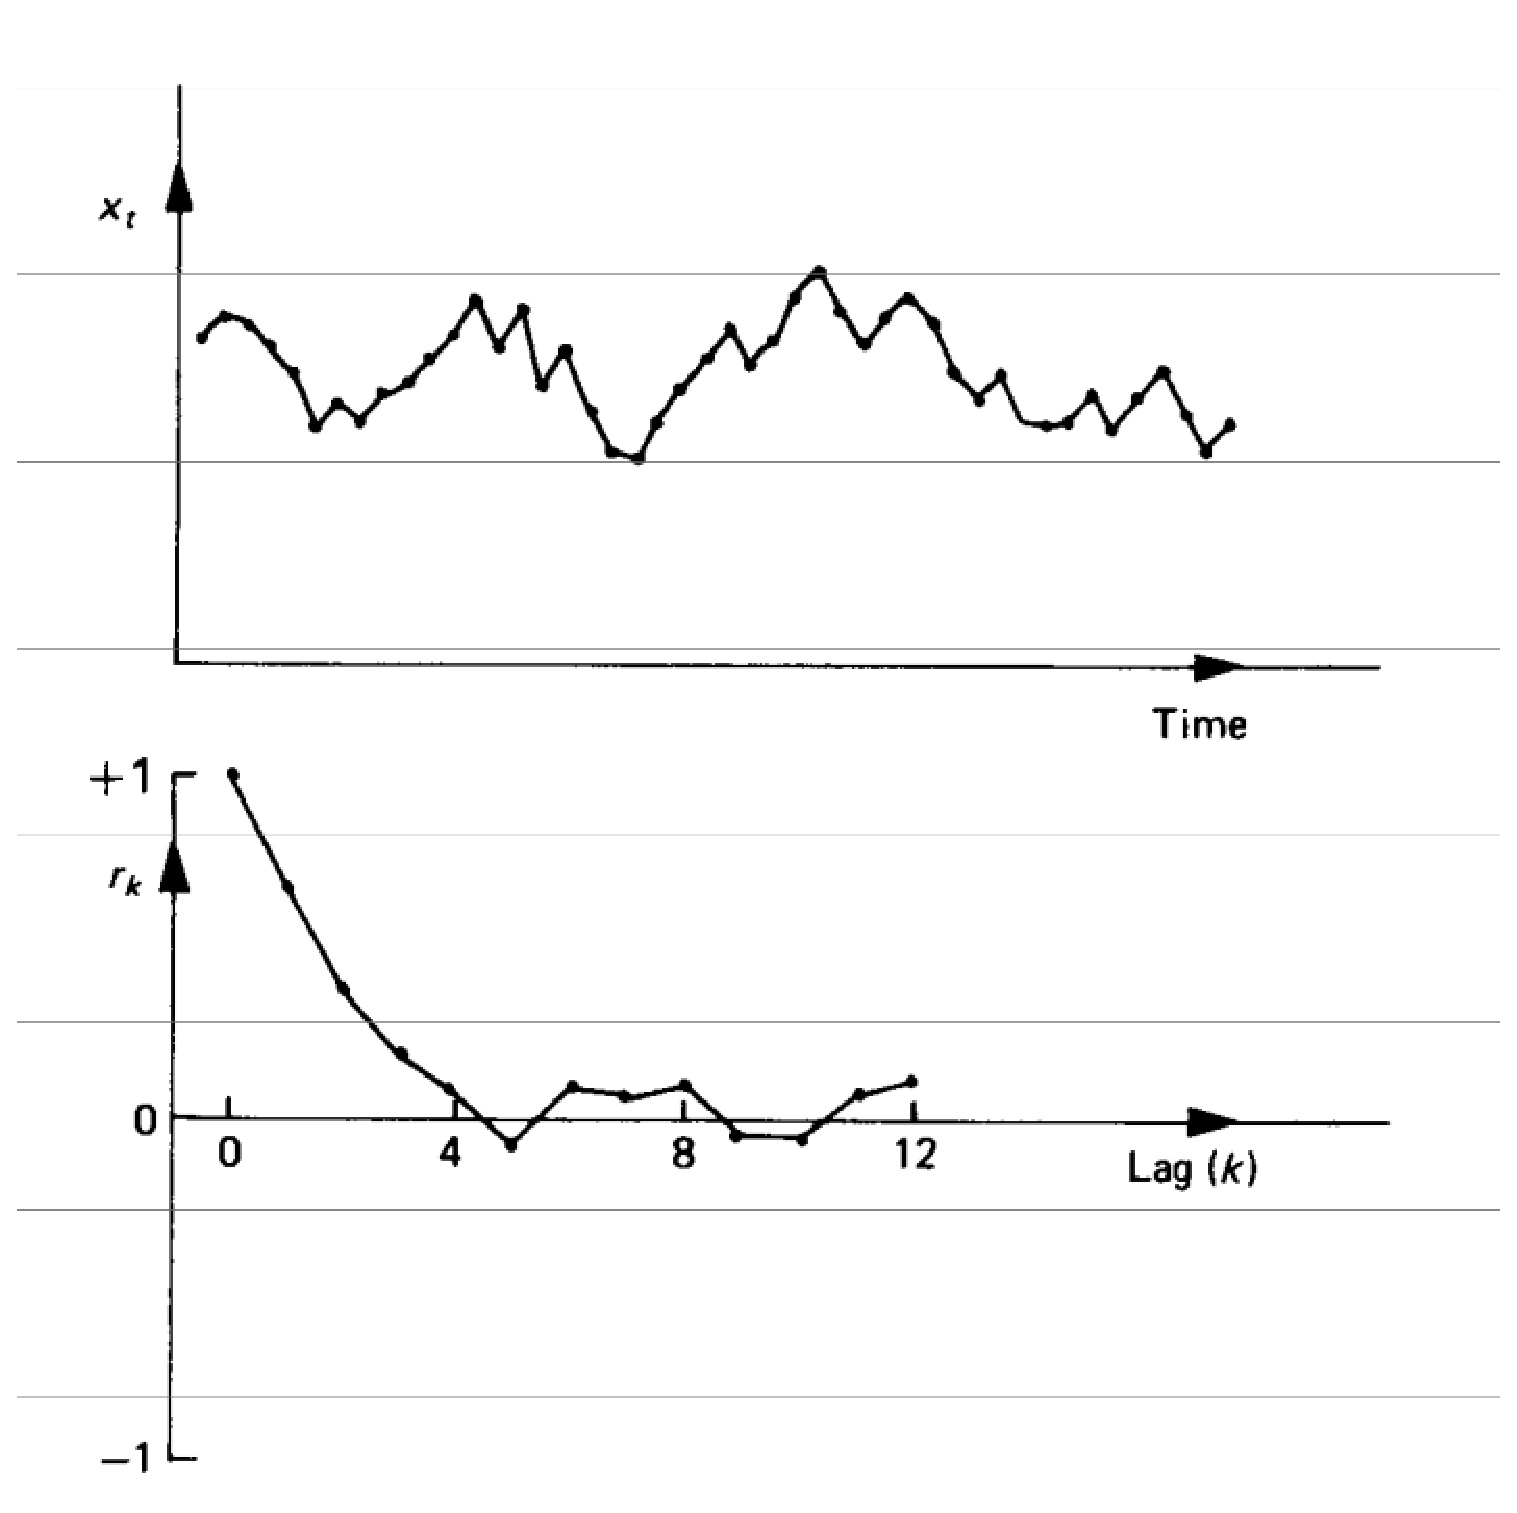
\includegraphics[scale = 0.40]{pictures/figure_2_1.eps}
\caption{Časová řada s krátkodobou korelací a její korelogram}
\label{figure_2_1}
\end{figure}

\subsubsection{Alternující časová řada}

Alternující časová řada se vyznačuje tím, že se její pozorování střídavě nacházejí nad a pod její střední hodnotou. Pokud časová řada alternuje, má tendenci alternovat také autokorelační koeficient $r_k$, který s každým posunem mění znaménko.

\begin{figure}[htp]
\centering
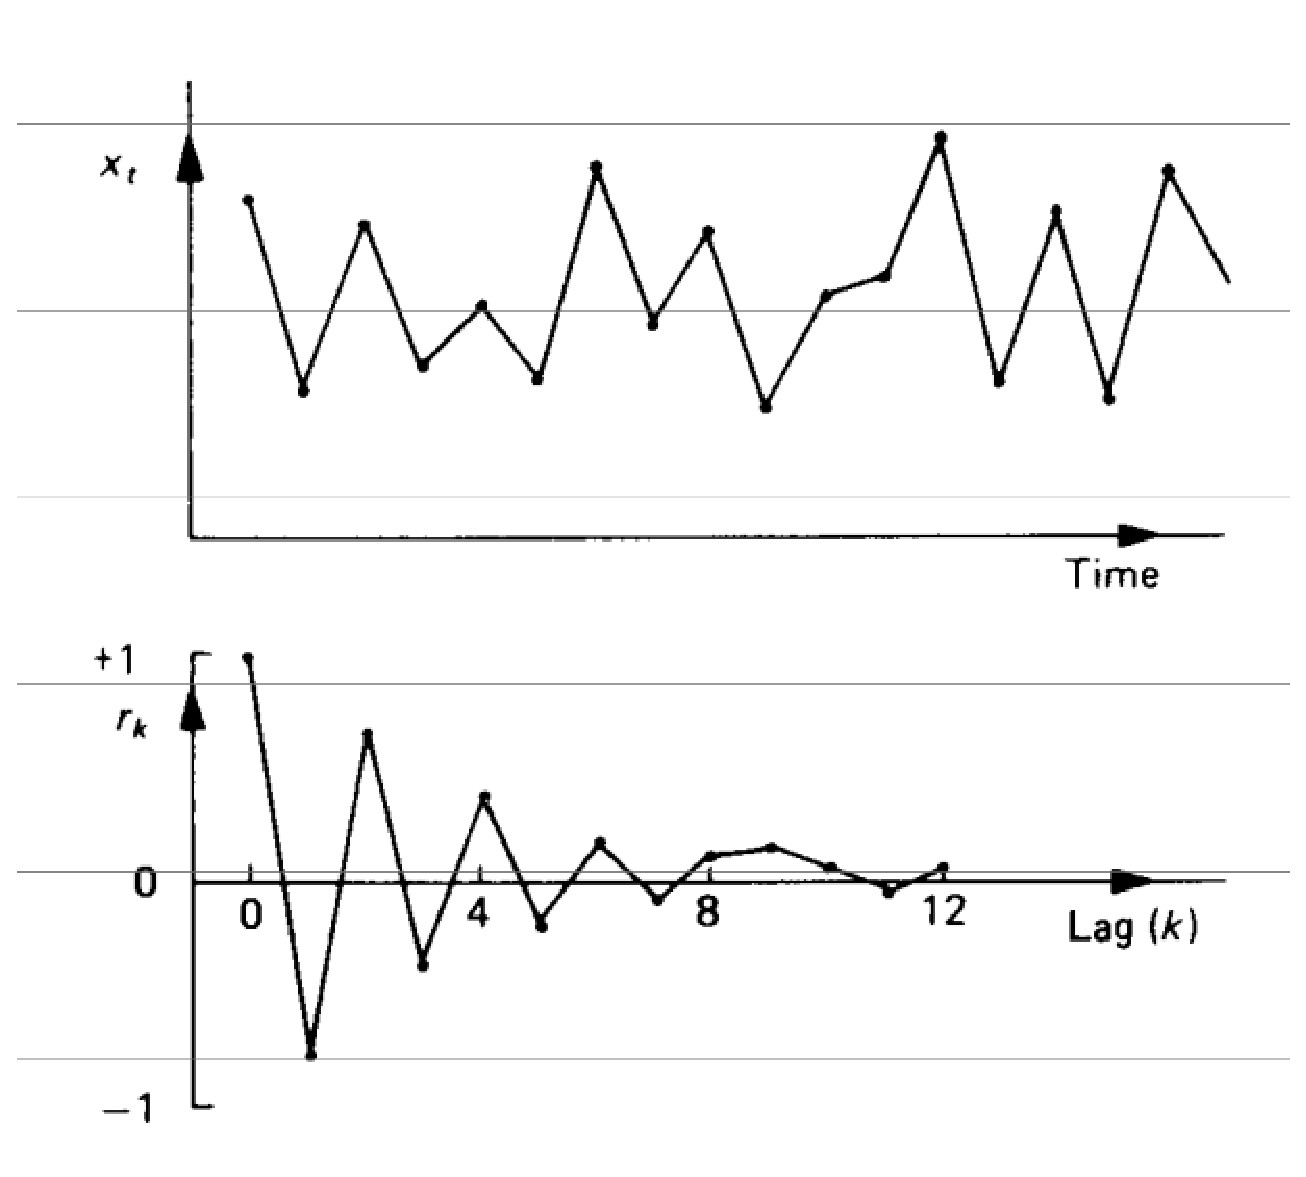
\includegraphics[scale = 0.40]{pictures/figure_2_2.eps}
\caption{Alternující časová řada a její korelogram}
\label{figure_2_2}
\end{figure}

\subsubsection{Časová řada s trendem}

Jestliže časová řada sleduje trend, neklesá hodnota autokorelačního koeficientu k nule s výjimkou velmi vysokého $k$. Z korelogramu tak lze vyčíst jen velmi málo, protože trend dominuje nad všemi ostatními vlastnostmi časové řady. Autokorelační funkce $\{r_k\}$ proto dává smysl pouze v případě stacionárních časových řad.

\begin{figure}[htp]
\centering
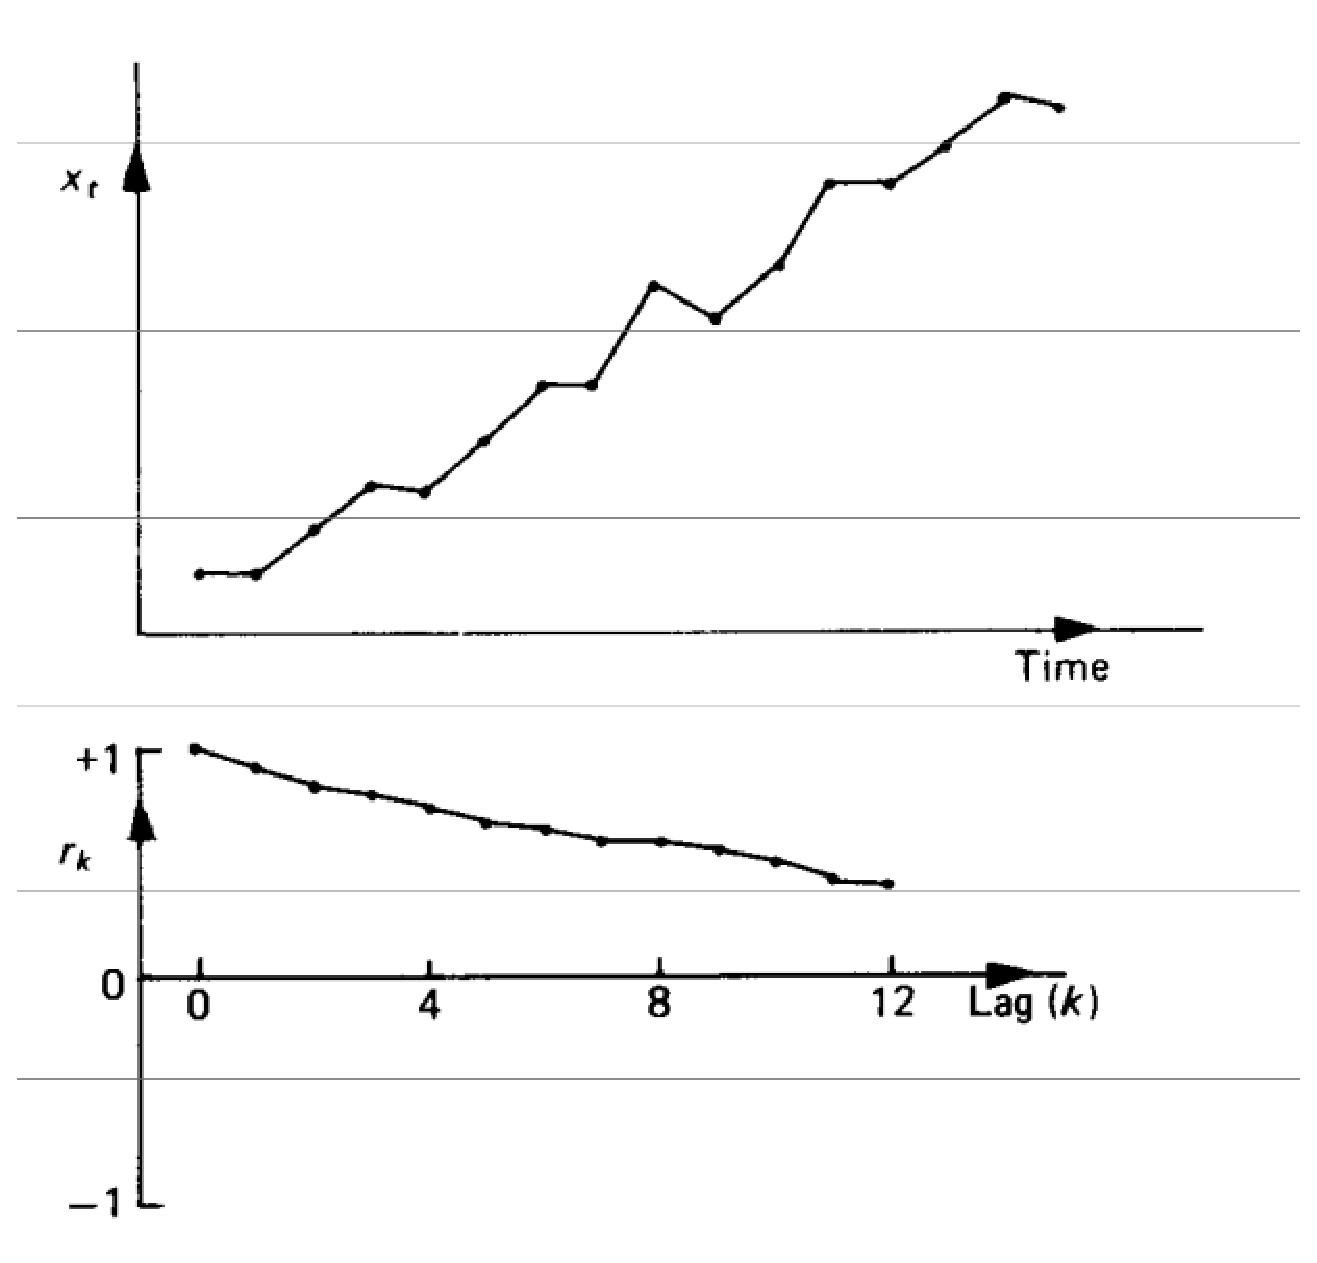
\includegraphics[scale = 0.40]{pictures/figure_2_3.eps}
\caption{Nestacionární časová řada a její korelogram}
\label{figure_2_3}
\end{figure}

\subsubsection{Časová řada se sezónní fluktuací}

Pokud časová řada obsahuje sezónní fluktuaci, osciluje také její korelogram a to se stejnou frekvencí. Obecně tak platí, že pokud $x_t$ má tvar sinusoidy, má tento tvar také $r_k$. Stejně jako ve výše uvedeném příkladě poskytuje korelogram řady se sezónní fluktuací pouze omezenou informaci. Nicméně po odstranění sezónnosti může korelogram určitou informaci poskytnout. Např. obrázek (\ref{figure_2_4}) představuje korelogramy vývoje měsíční teploty. Horní korelogram je zkonstruován na původní časové řadě; dolní korelogram pak na časové řadě očištěné o sezónnost. Z druhého korelogramu je patrné, že první tři autokorelační koeficienty jsou významně odlišné od nuly. Jinými slovy, pokud je určitý měsíc nadprůměrně chladný, je zpravidla následován dalšími dvěma chladnými měsíci a obráceně.

\begin{figure}[htp]
\centering
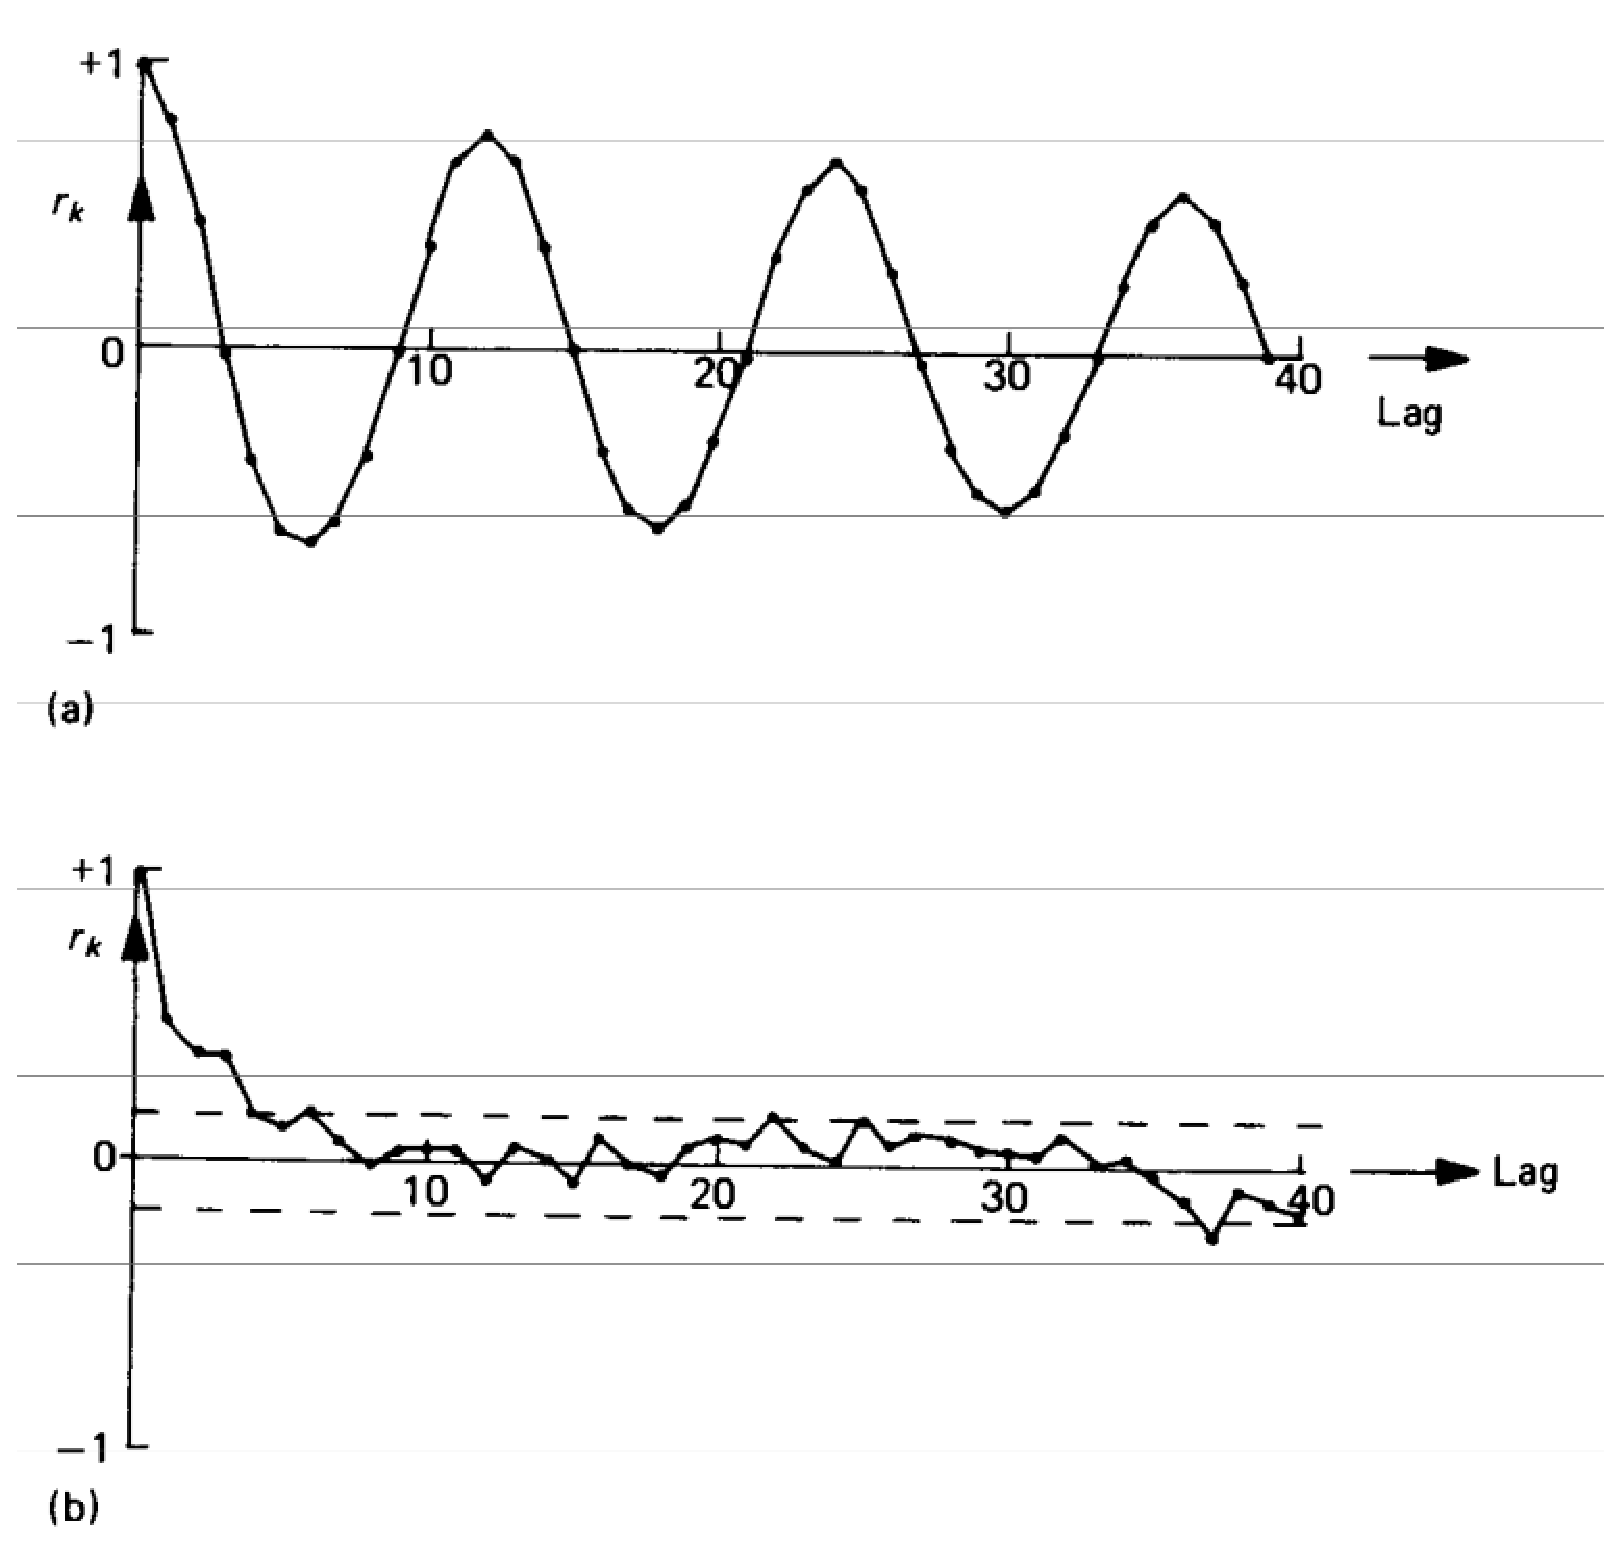
\includegraphics[scale = 0.40]{pictures/figure_2_4.eps}
\caption{Časová řada měsíčních teplot: (a) korelogram původní časové řady; (b) korelogram po odstranění sezónnosti (přerušovaná čára představuje $\pm \frac{2}{\sqrt{N}}$)}
\label{figure_2_4}
\end{figure}

\subsubsection{Odlehlá pozorování}

Pokud časová řada obsahuje jedno nebo vícero odlehlých pozorování, může to mít významný dopad na její korelogram. Např. pokud časová řada obsahuje jedno odlehlé pozorování, pak graf porovnávající $x_t$ a $x_{t + k}$ bude zahrnovat dva ``extrémní" body, které budou celkovou korelaci ``stlačovat" k nule. S narůstajícím počtem odlehlých pozorování se pak tento problém dále prohlubuje.